\begin{minipage}[c]{.45\linewidth} 
\Large \textbf{\textsf{NOM4 Prenom4}} 
 
 \normalsize Note harmonisée 7.41/20 
 
Rang 7
 
Note brute 7.41/20 
 
Moyenne classe harmonisée 5.77/20 
 
Commentaires : 
c4 
\end{minipage}\hfill 
\begin{minipage}[c]{.45\linewidth}  
\begin{center}
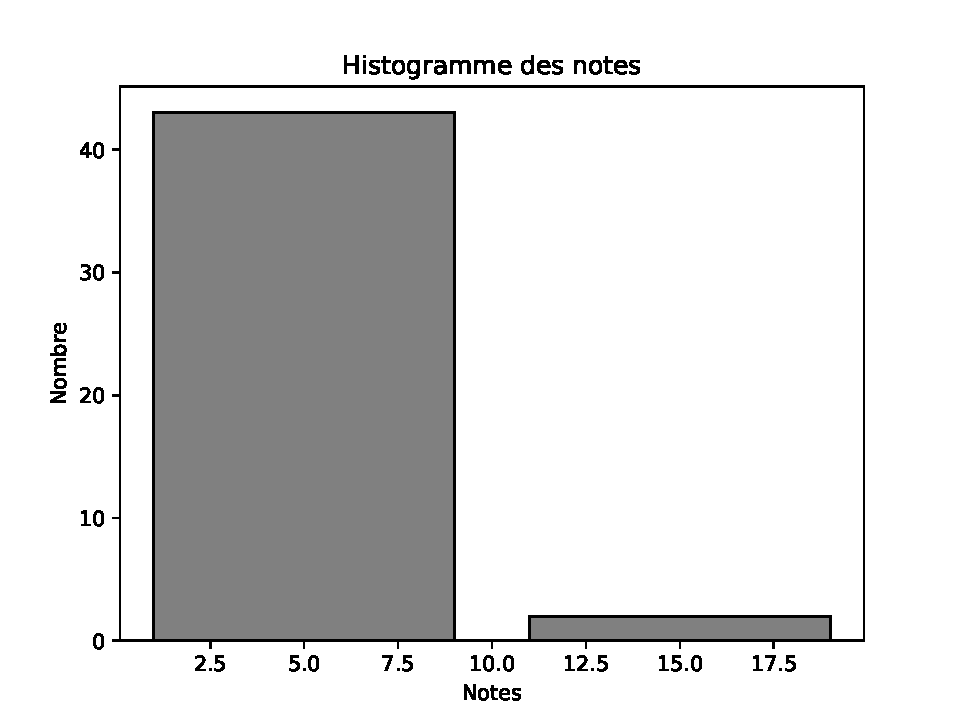
\includegraphics[width=.8\linewidth]{../histo.pdf} 
\end{center}
\end{minipage}
\footnotesize 
\begin{center} 
\begin{tabular}{|c|c|c|c||c|c|c|c||c|c|c|c||c|c|c|c|} 
\hline \textbf{Qu} & \textbf{Coef} & \textbf{Comp} & \textbf{/5} & \textbf{Qu} & \textbf{Coef} & \textbf{Comp} & \textbf{/5} & \textbf{Qu} & \textbf{Coef} & \textbf{Comp} & \textbf{/5} & \textbf{Qu} & \textbf{Coef} & \textbf{Comp} & \textbf{/5} \\ 
\hline 
\hline 
1 & 1 & Mod2.C1 & 5 & 18 & 1 & Mod2.C1 & 0 & 2 & 2 & An3.C1.SF7 & 5 & 19 & 1 & An3.C1 & 2 \\ \hline 
2 & 2 & Mod2.C1 & 5 & 19 & 1 & Mod2.C1 & 2 & 3 & 1 & An3.C12 & 5 & 20 & 1 & An3.C1.SF7 & 0 \\ \hline 
3 & 1 & Mod2.C1 & 5 & 20 & 1 & Mod2.C1 & 0 & 4 & 2 & An3.C1 & 0 & 21 & 1 & An3.C12 & 0 \\ \hline 
4 & 2 & Mod2.C1 & 0 & 21 & 1 & Mod2.C1 & 0 & 5 & 2 & An3.C1.SF7 & 2.5 & 22 & 1 & An3.C1 & 0 \\ \hline 
5 & 2 & Mod2.C1 & 2.5 & 22 & 1 & Mod2.C1 & 0 & 6 & 1 & An3.C12 & 5 & 23 & 2 & An3.C1.SF7 & 4 \\ \hline 
6 & 1 & Mod2.C1 & 5 & 23 & 2 & Mod2.C1 & 4 & 7 & 3 & An3.C1 & 0 & 24 & 3 & An3.C12 & 3.5 \\ \hline 
7 & 3 & Mod2.C1 & 0 & 24 & 3 & Mod2.C1 & 3.5 & 8 & 1 & An3.C1.SF7 & 2 & 25 & 1 & Mod2.C1 & 1 \\ \hline 
8 & 1 & Mod2.C1 & 2 & 25 & 1 & Mod2.C1 & 1 & 9 & 1.5 & An3.C12 & 0 & 26 & 1 & Mod2.C1 & 1 \\ \hline 
9 & 1.5 & Mod2.C1 & 0 & 26 & 1 & Mod2.C1 & 1 & 10 & 3 & An3.C1 & 3 & 27 & 1 & Mod2.C1 & 0 \\ \hline 
10 & 3 & Mod2.C1 & 3 & 27 & 1 & Mod2.C1 & 0 & 11 & 1 & An3.C1.SF7 & 0 & 28 & 1 & Mod2.C1 & 0.5 \\ \hline 
11 & 1 & Mod2.C1 & 0 & 28 & 1 & Mod2.C1 & 0.5 & 12 & 3 & An3.C12 & 3 & 29 & 4 & Mod2.C1 & 0 \\ \hline 
12 & 3 & Mod2.C1 & 3 & 29 & 4 & Mod2.C1 & 0 & 13 & 1.5 & An3.C1 & 1 & 30 & 1 & Mod2.C1 & 4 \\ \hline 
13 & 1.5 & Mod2.C1 & 1 & 30 & 1 & Mod2.C1 & 4 & 14 & 0.5 & An3.C1.SF7 & 0 & 31 & 1 & Mod2.C1 & 5 \\ \hline 
14 & 0.5 & Mod2.C1 & 0 & 31 & 1 & Mod2.C1 & 5 & 15 & 2 & An3.C12 & 0 & 32 & 1 & Mod2.C1 & 5 \\ \hline 
15 & 2 & Mod2.C1 & 0 & 32 & 1 & Mod2.C1 & 5 & 16 & 2 & An3.C1 & 0 & 33 & 1 & Mod2.C1 & 5 \\ \hline 
16 & 2 & Mod2.C1 & 0 & 33 & 1 & Mod2.C1 & 5 & 17 & 1 & An3.C1.SF7 & 0 &  &  &  &  \\ \hline 

17 & 1 & Mod2.C1 & 0 & 1 & 1 & An3.C1 & 5 & 18 & 1 & An3.C12 & 0 &  &  &  &  \\ \hline 

\end{tabular} 
\end{center} 
\normalsize 
 
\footnotesize 
\begin{center} 
\begin{tabular}{|p{.7\linewidth}|c|} 
\hline 
Compétences  & Taux \\ \hline \hline 
Mod2.C1 -- Chaîne d’énergie et d'information&26 \% \\ \hline 
An3.C1 -- Architectures fonctionnelle et structurelle &36 \% \\ \hline 
An3.C1.SF7 -- Justifier le choix des constituants dédiés aux fonctions d’un système&53 \% \\ \hline 
An3.C12 -- Réversibilité de la chaîne d’énergie :&42 \% \\ \hline 
\end{tabular} 
\end{center} 
\normalsize 
 
